
%(BEGIN_QUESTION)
% Copyright 2010, Tony R. Kuphaldt, released under the Creative Commons Attribution License (v 1.0)
% This means you may do almost anything with this work of mine, so long as you give me proper credit

``Wet'' natural gas is mostly methane (CH$_{4}$) mixed with significant amounts of heavier hydrocarbon species such as ethane (C$_{2}$H$_{6}$), propane (C$_{3}$H$_{8}$), butane (C$_{4}$H$_{10}$), and pentane (C$_{5}$H$_{12}$) which condense into liquid at lower temperatures than methane.  A process for separating these heavier hydrocarbons from the chief component (methane) using compression and cooling is shown here:

$$\includegraphics[width=15.5cm]{i01863x01.eps}$$

Chilled gases enter the flash vessel, where methane rises and escapes in gaseous form, while all the other (heavier) hydrocarbon molecules condense into liquid and exit out the bottom.

\vskip 10pt

Suppose PIC-115 is a proportional-only controller, holding steadily and accurately to a setpoint value of 107 PSI with a valve position of 41\%.  How will this controller respond to a sudden change in natural gas composition that is much {\it drier} than usual, assuming the same total flowrate (as indicated by FT-110) as before?  Be as specific as you can in your answer!

\vskip 20pt \vbox{\hrule \hbox{\strut \vrule{} {\bf Suggestions for Socratic discussion} \vrule} \hrule}

\begin{itemize}
\item{} Explain the purpose of the heat exchangers in this P\&ID, especially the two exchanging heat between the incoming (compressed) gas and the products coming off the top and bottom of the flash vessel.
\item{} Identify and explain the purpose of the ``PSV'' valve in this diagram.
\item{} Suppose the operator of this process notices a consistent offset between PV and SP for controller PIC-115, with SP = 60\% and PV = 65\%.  Describe steps the operator can take to eliminate this offset and get the PV equal to 60\%.
\end{itemize}

\underbar{file i01863}
%(END_QUESTION)





%(BEGIN_ANSWER)

``Drier'' natural gas entering this system means more methane and less of the heavier hydrocarbons.  This will result in less liquid drained off the bottom of the flash vessel, and more methane gas vented off the top.  In order to hold the flash vessel pressure steady, PIC-115 will have to ``open up'' its control valve just a bit to vent the additional methane gas.  However, since it is a proportional-only controller, it will be incapable of settling exactly back on the setpoint value of 107 PSI and instead will settle at some higher value (i.e. proportional-only offset).

%(END_ANSWER)





%(BEGIN_NOTES)

\vskip 20pt \vbox{\hrule \hbox{\strut \vrule{} {\bf Virtual Troubleshooting} \vrule} \hrule}

This question is a good candidate for a ``Virtual Troubleshooting'' exercise.  Presenting the diagram to students, you first imagine in your own mind a particular fault in the system.  Then, you present one or more symptoms of that fault (something noticeable by an operator or other user of the system).  Students then propose various diagnostic tests to perform on this system to identify the nature and location of the fault, as though they were technicians trying to troubleshoot the problem.  Your job is to tell them what the result(s) would be for each of the proposed diagnostic tests, documenting those results where all the students can see.

During and after the exercise, it is good to ask students follow-up questions such as:

\begin{itemize}
\item{} What does the result of the last diagnostic test tell you about the fault?
\item{} Suppose the results of the last diagnostic test were different.  What then would that result tell you about the fault?
\item{} Is the last diagnostic test the best one we could do?
\item{} What would be the ideal order of tests, to diagnose the problem in as few steps as possible?
\end{itemize}


%INDEX% Control, proportional: proportional-only offset
%INDEX% Process: "wet" natural gas separation

%(END_NOTES)


